\documentclass[12pt]{beamer}

\hypersetup{colorlinks=true,linkcolor = blue}
\usetheme{Warsaw}

\usepackage[utf8]{inputenc}
\usepackage[russian,english]{babel}
\usepackage[T2A]{fontenc}

\usepackage{hyperref}
\usepackage[final]{listings}
\usepackage{breakurl}
\usepackage{cite}
\usepackage{perpage}

\def\Url\Breaks{\do\/\do-}

\lstset{
  frame=single,
  breaklines=true,
  basicstyle=\tiny,
  postbreak=\raisebox{0ex}{\ensuremath{\hookrightarrow\space}},
  numbers=left
}

\MakePerPage{footnote}

\title{Operating Systems}
\subtitle{Threads Synchronization}
\author{Me}
\date{\today}

\begin{document}

  \begin{frame}
    \titlepage
  \end{frame}

  \begin{frame}
\frametitle{План лекции}
\begin{itemize}
  \item Устройства хранения. Планирование IO.
  \item Файловая система из userspace.
  \item Пример: FAT.
  \item Пример: FFS.
  \item Индексные структуры данных. B-деревья и их вариации.
  \item Надежность файловых систем. Fsck, журналирование и COW.
\end{itemize}
\end{frame}

  \begin{frame}
\frametitle{Конкурентное исполнение}
\begin{figure}
  \centering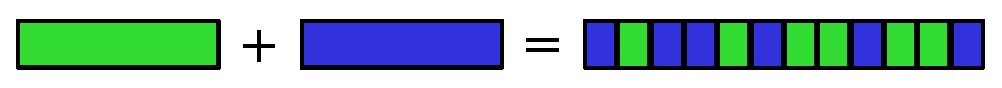
\includegraphics[width=.8\linewidth]{concurrency}
  \caption{Concurrent Execution}
\end{figure}

Конкурентное исполнение - исполняющиеся участки кода накладываются друг на
друга произвольным образом

\begin{itemize}
  \item вы не должны делать никаких предположений о порядке наложения;
  \item произвольный порядок ведет к произвольному доступу к общим ресурсам;
\end{itemize}
\end{frame}

\begin{frame}
\frametitle{Конкурентное исполнение}
\framesubtitle{Источники конкурентности}

\begin{itemize}
  \item<1-> много агентов исполняющих код:
        \begin{itemize}
          \item Hyper Threading, SMP, NUMA (shared memory);
          \item cluster nodes (shared storage);
        \end{itemize}
  \item<2-> прерывания - прерывают один код и запускают исполнение другого;
  \item<3-> сигналы - userspace аналог прерываний.
\end{itemize}
\end{frame}

\begin{frame}[fragile]
\frametitle{Конкурентное исполнение}
\framesubtitle{Состояние гонки}

\begin{columns}[T]
  \begin{column}{.45\linewidth}
    \begin{lstlisting}
int cnt;

void foo(void)
{
  ++cnt;
}
    \end{lstlisting}
  \end{column}
  \begin{column}{.45\linewidth}
    \begin{lstlisting}
extern int cnt;

void bar(void)
{
  ++cnt;
}
    \end{lstlisting}
  \end{column}
\end{columns}
\end{frame}

\begin{frame}[fragile]
\frametitle{Конкурентное исполнение}
\framesubtitle{Состояние гонки}

\begin{columns}[T]
  \begin{column}{.45\linewidth}
    \begin{lstlisting}
  .global cnt
cnt:
  .int 0

foo:
  mov cnt, %rax
  inc %rax
  mov %rax, cnt
  ret
    \end{lstlisting}
  \end{column}
  \begin{column}{.45\linewidth}
    \begin{lstlisting}
  .extern cnt

bar:
  mov cnt, %rax
  inc %rax
  mov %rax, cnt
  ret
    \end{lstlisting}
  \end{column}
\end{columns}
\end{frame}

\begin{frame}
\frametitle{Взаимное исключение}

Взаимное исключение (Mutual Exclusion) - позволяет оградить критическую секцию,
чтобы предотвратить конкуренции

\begin{itemize}
  \item lock и unlock - ограничивают критическую секции в начале и конце
        соответственно;
  \item только один поток исполнения может находиться в критической секции
        \begin{itemize}
          \item lock не вернет управление, до тех пор, пока поток в критической
                секции не сделает unlock;
        \end{itemize}
  \item если в критической секции не находится поток, то из нескольких
        конкурирующих lock-ов, как минимум один будет успешным;
\end{itemize}
\end{frame}

\begin{frame}
\frametitle{Взаимное исключение}

Мы можем считать, что
\begin{itemize}
  \item поток выйдет из критической секции за конечное время
        \begin{itemize}
          \item поток не зависнет и не упадет внутри критической секции;
        \end{itemize}
\end{itemize}

\onslide<2->{Мы не можем делать предположений о
\begin{itemize}
  \item скорости работы потока
        \begin{itemize}
          \item время нахождения в критической секции конечно, но ограничение
                сверху нам не известно;
        \end{itemize}
  \item взаимной скорости работы потоков
        \begin{itemize}
          \item мы не можем считать, что один поток быстрее/медленнее другого или
                что их скорости равны
        \end{itemize}
\end{itemize}}
\end{frame}

\begin{frame}[fragile]
\frametitle{Реализация взаимного исключения}
\framesubtitle{Глобальный флаг}

\begin{columns}[T]
  \begin{column}{.45\linewidth}
    \begin{lstlisting}
extern int claim1;
int claim0;

void lock0()
{
  claim0 = true;
  while (claim1);
}

void unlock0(void)
{
  claim0 = false;
}
    \end{lstlisting}
  \end{column}
  \begin{column}{.45\linewidth}
    \begin{lstlisting}
extern int claim0;
int claim1;

void lock1(void)
{
  claim1 = true;
  while (claim0);
}

void unlock1(void)
{
  claim1 = false;
}
    \end{lstlisting}
  \end{column}
\end{columns}
\end{frame}

\begin{frame}
\frametitle{Реализация взаимного исключения}
\framesubtitle{Глобальный флаг}

Следующее расписание приводит к deadlock-у:
\begin{enumerate}
  \item Thread 0, line 6;
  \item Thread 1, line 6;
  \item Thread 0, line 7 (Thread 0 завис на этой строке);
  \item Thread 1, line 7 (Thread 1 завис на этой строке);
\end{enumerate}
\end{frame}

\begin{frame}[fragile]
\frametitle{Реализация взаимного исключения}
\framesubtitle{Глобальный порядок}

\begin{columns}[T]
  \begin{column}{.45\linewidth}
    \begin{lstlisting}
int turn;

void lock0(void)
{
  while (turn != 0);
}

void unlock0(void)
{
  turn = 1;
}
    \end{lstlisting}
  \end{column}
  \begin{column}{.45\linewidth}
    \begin{lstlisting}
extern int turn;

void lock1(void)
{
  while (turn != 1);
}

void unlock0(void)
{
  turn = 0;
}
    \end{lstlisting}
  \end{column}
\end{columns}
\end{frame}

\begin{frame}
\frametitle{Реализация взаимного исключения}
\framesubtitle{Глобальный порядок}

Расписание приводящее к проблемам:
\begin{enumerate}
  \item Thread 1, line 5 (Thread 1 завис на этой строке);
  \item Thread 0 - умер (решил не заходить в критическую секцию);
\end{enumerate}
\onslide<2->{Да, оно довольно короткое...}
\end{frame}

\begin{frame}[fragile]
\frametitle{Реализация взаимного исключения}
\framesubtitle{Соберем все в кучу}

\begin{columns}[T]
  \begin{column}{.45\linewidth}
    \begin{lstlisting}
extern int claim1;
int claim0;
int turn;

void lock0(void)
{
  claim0 = true;
  turn = 1;

  while (claim1 && turn == 1);
}

void unlock0(void)
{
  claim0 = false;
}
    \end{lstlisting}
  \end{column}
  \begin{column}{.45\linewidth}
    \begin{lstlisting}
extern int claim0;
extern int turn;
int claim1;

void lock1(void)
{
  claim1 = true;
  turn = 0;

  while (claim0 && turn == 0);
}

void unlock1(void)
{
  claim1 = false;
}
    \end{lstlisting}
  \end{column}
\end{columns}
\end{frame}

\begin{frame}
\frametitle{Реализация взаимного исключения}
\framesubtitle{Алгоритм Петтерсона}

\emph{Доказательство взаимного исключения:}
\begin{itemize}
  \item пусть сразу два потока находятся в критической секции:
        \begin{itemize}
          \item turn принимает одно из двух значений: 0 или 1; для
                определенности пусть это будет 0, т. е. последним в turn
                записывал поток 1;
          \item claim0 и claim1 оба равны true;
        \end{itemize}
  \item к моменту проверки условия цикла потоком 1 имеем:
        \begin{itemize}
          \item turn равен 0;
          \item claim0 равен true;
          \item но в этом случае поток 1 должен зависнуть в цикле до изменения
                turn или claim0 - противоречие;
        \end{itemize}
\end{itemize}
\end{frame}

\begin{frame}
\frametitle{Реализация взаимного исключения}
\framesubtitle{Алгоритм Петтерсона}

\emph{Доказательство наличия прогресса:} пусть поток 0 пытается войти в
свободную критическую секцию:
\begin{itemize}
  \item<1-> поток 0 в 10 строке видит claim1 == true:
        \begin{itemize}
          \item поток 0 видит turn == 0, поток 0 входит в критическую секцию;
          \item поток 0 видит turn == 1, возможны два случая:
                \begin{itemize}
                  \item поток 1 выполнил строку 8, поток 0 перезаписал turn -
                        поток 1 входит в критическую секцию;
                  \item поток 1 собирается выполнить строку 8 - поток 0 войдет в
                        критическую секцию, после того как поток 1 выполнит
                        строку 8;
                \end{itemize}
        \end{itemize}
  \item<2> поток 0 видит claim1 == false - поток 0 входит в критическую секцию;
\end{itemize}
\end{frame}

\begin{frame}[fragile]
\frametitle{Реализация взаимного исключения}
\framesubtitle{Алгоритм Петтерсона для N потоков}

\begin{lstlisting}
int flag[N];
int turn[N - 1];

void lock(int i)
{
  for (int count = 0; count < N - 1; ++count) {
    flag[i] = count + 1;
    turn[count] = i;

    int found = true;
    while (turn[count] == i && found) {
      found = false;
      for (int k = 0; !found && k != N; ++k) {
        if (k == i) continue;
        found = flag[k] > count;
      }
    }
  }
}

void unlock(int i)
{
  flag[i] = 0;
}
\end{lstlisting}
\end{frame}

\begin{frame}
\frametitle{Реализация взаимного исключения}
\framesubtitle{Честность Алгоритма Петтерсона}

\only<1>{Рассмотрим пример на 3 потоках. Начальное состояние:
\begin{itemize}
  \item flag[3] = \{0, 0, 0\};
  \item turn[2] = \{0, 0\};
\end{itemize}}
\only<1>{Поток 0 пытается войти в критическую секцию (count = 0):
\begin{itemize}
  \item flag[3] = \{1, 0, 0\};
  \item turn[2] = \{0, 0\};
\end{itemize}}
\only<2>{Поток 1 пытается войти в критическую секцию (count = 0):
\begin{itemize}
  \item flag[3] = \{1, 1, 0\};
  \item turn[2] = \{1, 0\};
\end{itemize}}
\only<3>{Поток 2 пытается войти в критическую секцию (count = 0):
\begin{itemize}
  \item flag[3] = \{1, 1, 1\};
  \item turn[2] = \{2, 0\};
\end{itemize}}
\only<4>{Поток 1 пытается войти в критическую секцию (count = 1):
\begin{itemize}
  \item flag[3] = \{1, 2, 1\};
  \item turn[2] = \{2, 1\};
\end{itemize}}
\only<5>{Поток 1 вошел в критическую секцию... И вышел из критической секции:
\begin{itemize}
  \item flag[3] = \{1, 0, 1\};
  \item turn[2] = \{2, 1\};
\end{itemize}}
\only<6>{Поток 1 пытается войти в критическую секцию (count = 0):
\begin{itemize}
  \item flag[3] = \{1, 1, 1\};
  \item turn[2] = \{1, 1\};
\end{itemize}}
\only<7>{Поток 2 пытается войти в критическую секцию (count = 1):
\begin{itemize}
  \item flag[3] = \{1, 1, 2\};
  \item turn[2] = \{1, 2\};
\end{itemize}}
\only<8>{Поток 2 вошел в критическую секцию... И вышел из критической секции:
\begin{itemize}
  \item flag[3] = \{1, 1, 0\};
  \item turn[2] = \{1, 2\};
\end{itemize}}
\only<9>{Поток 2 пытается войти в критическую секцию (count = 0):
\begin{itemize}
  \item flag[3] = \{1, 1, 1\};
  \item turn[2] = \{2, 2\};
\end{itemize}}
\only<10>{Поток 1 пытается войти в критическую секцию (count = 1):
\begin{itemize}
  \item flag[3] = \{1, 2, 1\};
  \item turn[2] = \{2, 1\};
\end{itemize}
Мы уже были в этом состоянии! А поток 0 так и не получил управление!}
\end{frame}

\begin{frame}
\frametitle{Реализация взаимного исключения}
\framesubtitle{Честность Алгоритма Петтерсона}

Как определить честность? Разделим lock на две части:
\begin{itemize}
  \item вход ($D$) - всегда завершается за известное конечное
        количество шагов;
  \item ожидание ($W$) - может потребовать неограниченное количество шагов;
\end{itemize}

\onslide<2->{Свойство $r$-ограниченного ожидания для двух потоков (0 и 1):
\begin{itemize}
  \item если $D_{0}^{k}$ ($k$-ый вход потока 0) предшествует $D_{1}^{j}$
        ($j$-ому входу потока 1);
  \item тогда $k$-ая критическая секция потока 0, предшествует $j+r$-ой
        критической секции потока 1;
\end{itemize}}

\onslide<3->{Алгоритм Петтерсона не обладает свойством $r$-ограниченного ожидания
ни для какого $r$.}
\end{frame}

\begin{frame}
\frametitle{Реализация взаимного исключения}
\framesubtitle{Алгоритм Пекарни (Л. Лэмпорт)}

\onslide<1->{Каждый поток при попытке входа выбирает себе число:
\begin{itemize}
  \item число определяет место в очереди;
  \item новое число выбирается так, чтобы оно было больше всех чисел в очереди;
\end{itemize}}

\onslide<2->{Как выбирать это число?
\begin{itemize}
  \item посмотреть на числа всех потоков и прибавить 1 к наибольшему;
  \item что если два потока выбирают число одновременно?
\end{itemize}}

\onslide<3->{Как использовать выбранное число?
\begin{itemize}
  \item если число наименьшее среди всех потоков выбравших число, то входим в
        критическую секцию;
\end{itemize}}
\end{frame}

\begin{frame}[fragile]
\frametitle{Реализация взаимного исключения}
\framesubtitle{Алгоритм Пекарни (Л. Лэмпорт)}

\begin{columns}[T]
  \begin{column}{.45\linewidth}
    \begin{lstlisting}
int flag[N];
int number[N];

int max(void)
{
  int rc = 0;

  for (int i = 0; i != N; ++i) {
    const int n = number[i];

    if (n > rc)
      rc = n;
  }

  return rc;
}

int less(int id0, int n0,
         int id1, int n1)
{
  if (n0 < n1)
    return true;
  if (n0 == n1 && id0 < id1)
    return true;
  return false;
}
    \end{lstlisting}
  \end{column}
  \begin{column}{.45\linewidth}
    \begin{lstlisting}
void lock(int i)
{
  flag[i] = true;
  number[i] = max() + 1;
  flag[i] = false;

  for (int j = 0; j != N; ++j) {
    if (j == i)
      continue;

    while (flag[j]);
    while (number[j] &&
           less(j, number[j],
                i, number[i]));
  }
}

void unlock(int i)
{
  number[i] = 0;
}
    \end{lstlisting}
  \end{column}
\end{columns}
\end{frame}

\begin{frame}
\frametitle{Реализация взаимного исключения}
\framesubtitle{Честность алгоритм Пекарни}

\begin{itemize}
  \item вход алгоритма пекарни ($D$) состоит из:
        \begin{itemize}
          \item выбора нового числа для потока;
        \end{itemize}
  \item если $D_{0}^{k}$ предшествует $D_{1}^{j}$, то число выбранное потоком 0
        на входе $k$, будет меньше числа, выбранного потоком 1 на входе $j$;
  \item<2-> т. е. поток 0 войдет в $k$-ую критическую секцию раньше, чем поток 1
        войдет в $j$-ую - $0$-ограниченное ожидание.
\end{itemize}
\end{frame}

  \begin{frame}
\frametitle{Out-of-order execution}

К сожалению, описанные подходы, как есть, не будут работать...
\begin{itemize}
  \item<2-> компилятору \emph{разрешено} переставлять инструкции:
        \begin{itemize}
          \item компилятор может делать с кодом все, что угодно, пока
                наблюдаемое поведение остается неизменным;
          \item кеширование, удаление "мертвого" кода, спекулятивные записи и
                чтения и многое другое
        \end{itemize}
  \item<3-> процессоры могут использовать оптимизации изменяющие порядок работы
        с памятью:
        \begin{itemize}
          \item store buffer - сохранение данных во временный буфер вместо
                кеша;
          \item invalidate queue - отложенный сброс линии кеша;
        \end{itemize}
\end{itemize}
\end{frame}

\begin{frame}
\frametitle{Оптимизации компилятора}

Компилятор подбирает оптимальный набор инструкций реализующий заданное
наблюдаемое поведение (осторожно C и C++):
\begin{itemize}
  \item обращения к volatile данным (чтение и запись);
  \item операции ввода/вывода (printf, scanf и тд).
\end{itemize}

\onslide<2->{Если компилятору не сообщить, то он не знает:
\begin{itemize}
  \item что переменная может модифицироваться в другом потоке;
  \item что переменную может читать другой поток;
  \item что порядок обращений к переменным важен;
\end{itemize}}
\end{frame}

\begin{frame}
\frametitle{Барьеры компилятора}

\begin{itemize}
  \item Чтобы сообщить компилятору о "побочных" эффектах работы с памятью
        нужно сделать эту память частью наблюдаемого поведения - использовать
        ключевое слово volatile;
        \begin{itemize}
          \item компилятору запрещено переставлять обращения к volatile
                данным, \emph{если они разделены точкой следования};
          \item компилятор может переставлять доступ к volatile данным с
                доступом к не volatile данным;
        \end{itemize}
\end{itemize}
\end{frame}

\begin{frame}[fragile]
\frametitle{Барьеры компиялтора}

\begin{columns}[T]
  \begin{column}{.45\linewidth}
    \begin{lstlisting}
struct some_struct {
  int a, b, c;
};

struct some_struct * volatile public;

void foo(void)
{
  struct some_struct *ptr = alloc_some_struct();

  ptr->a = 1;
  ptr->b = 2;
  ptr->c = 3;
  // need something to prevent
  // reordering
  public = ptr;
}
    \end{lstlisting}
  \end{column}
  \begin{column}{.45\linewidth}
    \begin{lstlisting}
void bar(void)
{
  while (!public);
  // and here too
  assert(public->a == 1);
  assert(public->b == 2);
  assert(public->c == 3);
}
    \end{lstlisting}
  \end{column}
\end{columns}
\end{frame}

\begin{frame}[fragile]
\frametitle{Барьеры компилятора}

Итого: volatile мало чем помогает, что делать? \\
Смотреть в документацию компилятора! Например, gcc предлагает
следующее решение:

\begin{lstlisting}
#define barrier() asm volatile ("" : : : "memory")
\end{lstlisting}
\end{frame}

\begin{frame}[fragile]
\frametitle{Барьеры компилятора}

\begin{columns}[T]
  \begin{column}{.45\linewidth}
    \begin{lstlisting}
struct some_struct {
  int a, b, c;
};

#define barrier() asm volatile ("" : : : "memory")
struct some_struct *public;

void foo(void)
{
  struct some_struct *ptr = alloc_some_struct();

  ptr->a = 1;
  ptr->b = 2;
  ptr->c = 3;
  barrier();
  public = ptr;
}
    \end{lstlisting}
  \end{column}
  \begin{column}{.45\linewidth}
    \begin{lstlisting}
void bar(void)
{
  while (!public);
  barrier();
  assert(public->a == 1);
  assert(public->b == 2);
  assert(public->c == 3);
}
    \end{lstlisting}
  \end{column}
\end{columns}
\end{frame}

\begin{frame}
\frametitle{Когерентность процессорных кешей}

\begin{figure}
  \only<1>{\centering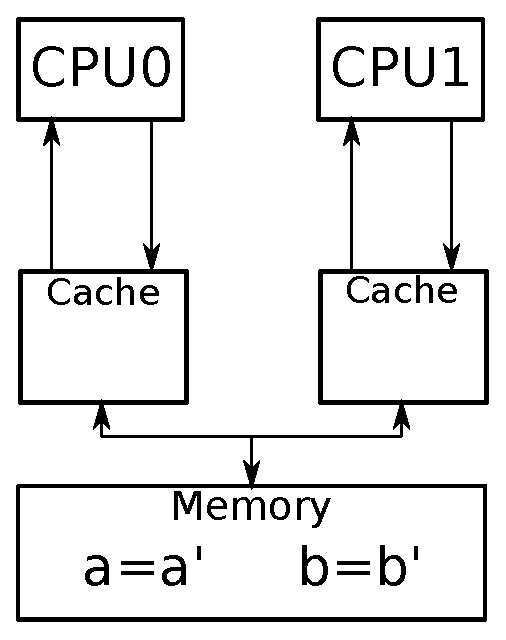
\includegraphics[height=.6\textheight]{cache-coh0}}
  \only<2>{\centering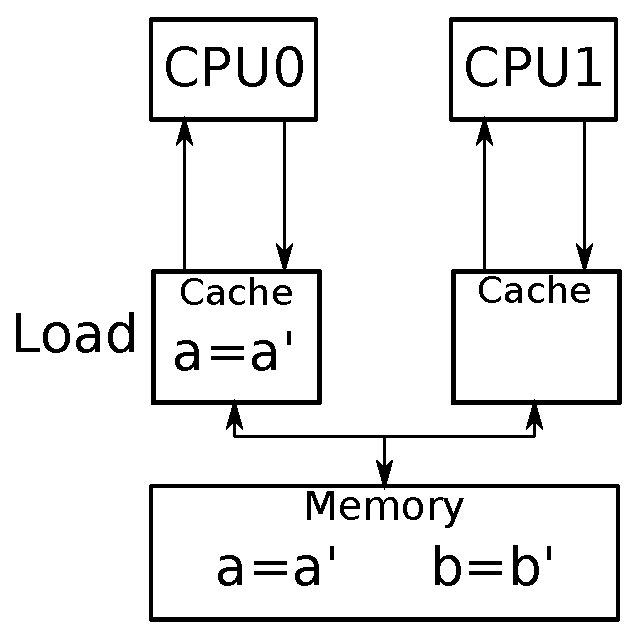
\includegraphics[height=.6\textheight]{cache-coh1}}
  \only<3>{\centering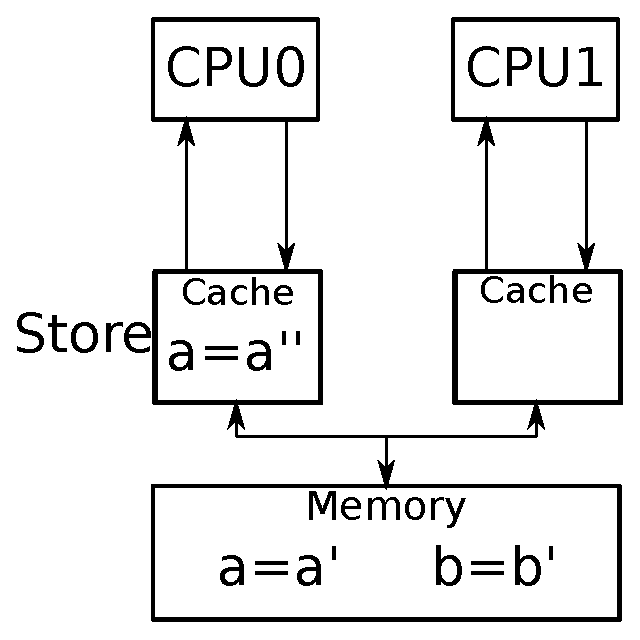
\includegraphics[height=.6\textheight]{cache-coh2}}
  \only<4>{\centering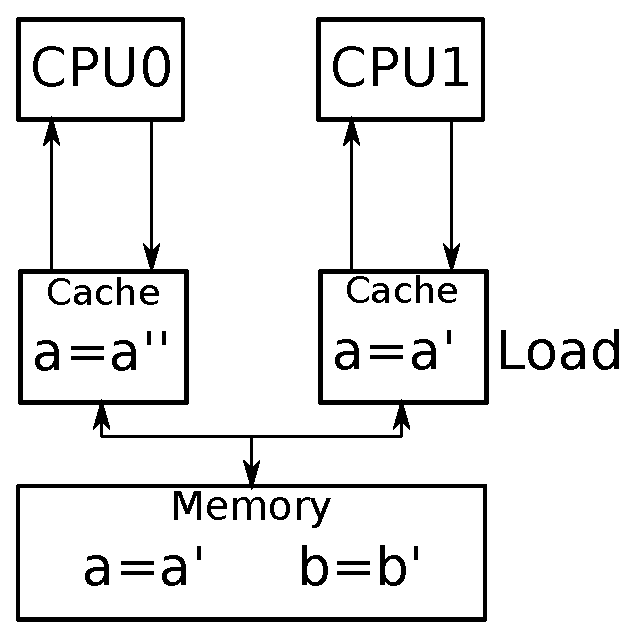
\includegraphics[height=.6\textheight]{cache-coh3}}
  \only<5>{\centering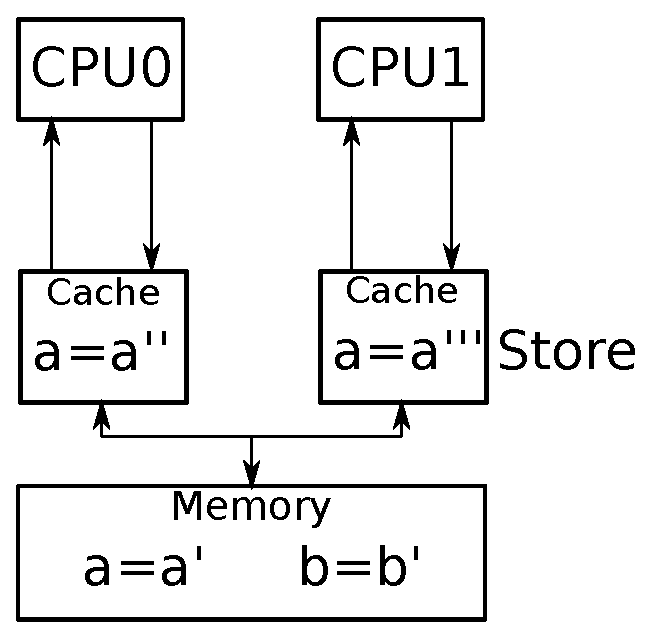
\includegraphics[height=.6\textheight]{cache-coh4}}
  \only<6>{\centering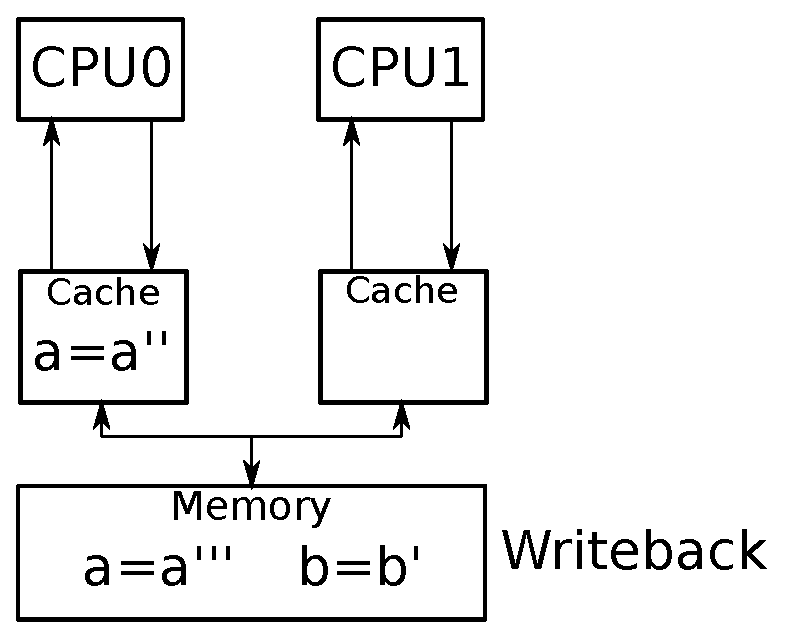
\includegraphics[height=.6\textheight]{cache-coh5}}
  \only<7>{\centering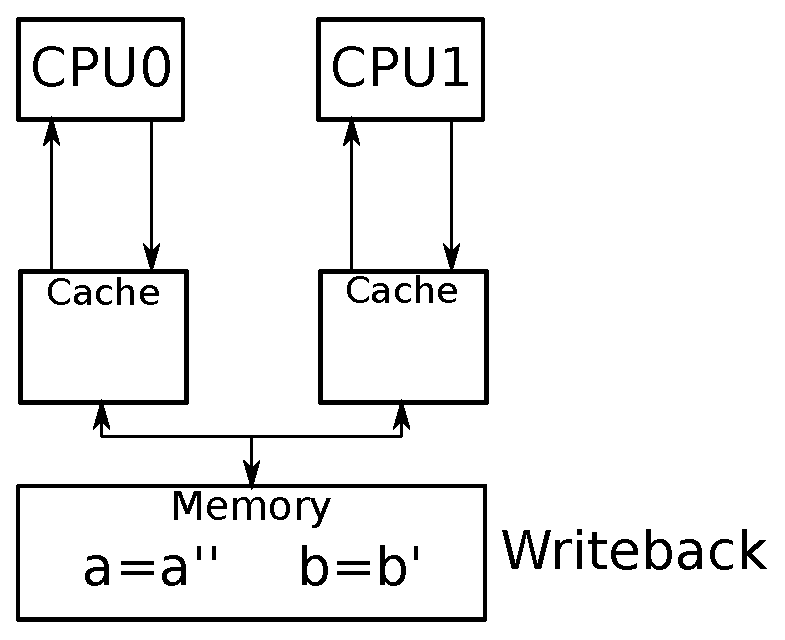
\includegraphics[height=.6\textheight]{cache-coh6}}
  \caption{Cache Incoherency}
\end{figure}
\end{frame}

\begin{frame}
\frametitle{Когерентность процессорных кешей}

Кеши должны находиться в согласованном состоянии (быть когерентными):
\begin{itemize}
  \item процессоры могут обмениваться сообщениями:
        \begin{itemize}
          \item можем считать, что сообщения передаются надежно;
          \item не можем полагаться на порядок доставки и обработки сообщений;
        \end{itemize}
  \item процессоры используют специальный протокол обеспечения когерентности:
        \begin{itemize}
          \item наверно, самый широко известный протокол - MESI (есть сомнения,
                что он используется без модификаций);
        \end{itemize}
\end{itemize}
\end{frame}

\begin{frame}
\frametitle{MESI}
MESI (Modified, Exclusive, Shared, Invalid) предполагает, что каждая линия кеша
находится в одном из четырех состояний:
\begin{itemize}
  \item Modified - кеш линия находится только в кеше данного процессора и она
        была записана (может отличаться от версии в памяти);
  \item Exclusive - кеш линия находится только в кеше данного процессора и она
        совпадает с копией в памяти;
  \item Shared - кеш линия находится в кеше данного процессора и возможно в
        кешах других процессоров, содержимое совпадает с памятью;
  \item Invalid - кеш линия не используется;
\end{itemize}
\end{frame}

\begin{frame}
\frametitle{MESI}
Перед тем как модифицировать данные процессор должен получить данные в
эксклюзивное пользование:
\begin{itemize}
  \item если несколько процессоров держат в кеше данные (Shared), то мы просим
        их сбросить данные;
  \item если другой процессор держит данные в кеше (Modified или Exclusive), то
        мы просим его передать нам данные
        \begin{itemize}
          \item контроллер памяти может увидеть передачу и обновить данные в
                памяти;
          \item или процессор может явно сбросить данные в память;
        \end{itemize}
  \item если никто не держит данные в кеше, то мы получаем их от контроллера
        памяти;
\end{itemize}
\end{frame}

\begin{frame}
\frametitle{Store Buffer}

\begin{figure}
  \centering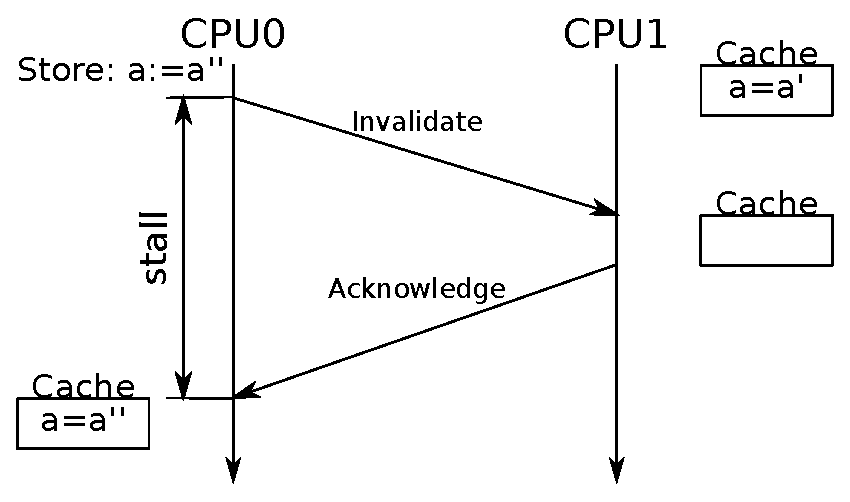
\includegraphics[width=.8\linewidth]{cache-store-stall}
  \caption{Cache Store Stall}
\end{figure}
\end{frame}

\begin{frame}
\frametitle{Store Buffer}

"Первая" запись данных приводит к ненужным остановкам конвейера:
\begin{itemize}
  \item другие процессоры должны сбросить данные из кеша;
  \item процессор должен дождаться от них подтверждения;
  \item<2-> но нам даже не нужно знать старое значение, если мы все равно его
        перезаписываем!
  \item<3-> заведем маленький кеш без поддержки когерентности (Store Buffer):
        \begin{itemize}
          \item первоначально запишем данные в него;
          \item когда придет подтверждение - сбросим данные в кеш;
        \end{itemize}
\end{itemize}
\end{frame}

\begin{frame}
\frametitle{Store Buffer}

\begin{figure}
  \centering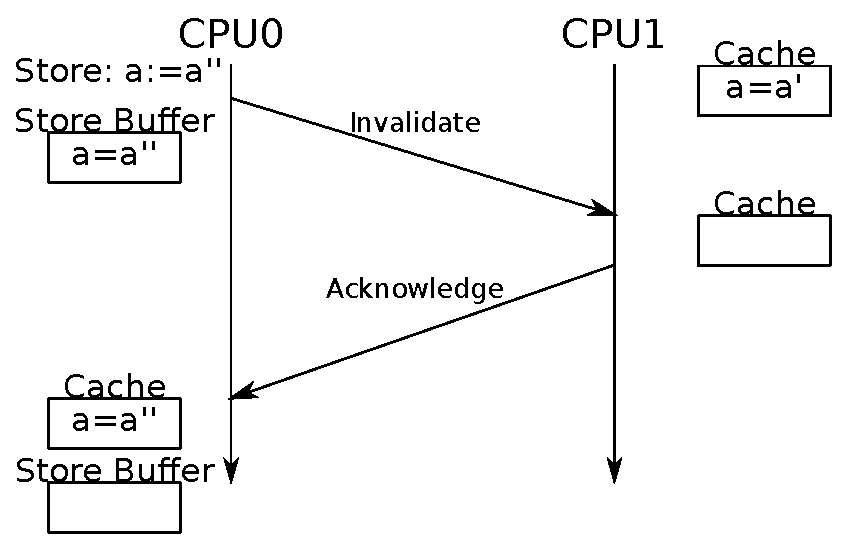
\includegraphics[width=.8\linewidth]{cache-store-buffer}
  \caption{Store Buffer}
\end{figure}
\end{frame}

\begin{frame}[fragile]
\frametitle{Memory Order Violation}

\begin{columns}[T]
  \begin{column}{.4\linewidth}
    \begin{lstlisting}
void foo(void)
{
  a = 1;
  barrier();
  b = 1;
}

void bar(void)
{
  while (b == 0)
    continue;
  barrier();
  assert(a == 1);
}
    \end{lstlisting}
  \end{column}
  \begin{column}{.6\linewidth}
    \begin{itemize}
      \item $a$ равна 0 и находится в кеше CPU1;
      \item $b$ равна 0 и находится в кеше CPU0;
      \item CPU0 исполняет foo и CPU1 исполняет bar;
    \end{itemize}
  \end{column}
\end{columns}
\end{frame}

\begin{frame}[fragile]
\frametitle{Memory Order Violation}

\begin{columns}[T]
  \begin{column}{.4\linewidth}
    \begin{lstlisting}[escapechar=!]
void foo(void)
{
  !\colorbox{hlcode}{a = 1;}!
  barrier();
  b = 1;
}

void bar(void)
{
  while (b == 0)
    continue;
  barrier();
  assert(a == 1);
}
    \end{lstlisting}
  \end{column}
  \begin{column}{.6\linewidth}
    \begin{itemize}
      \item CPU0 исполняет строку 3;
      \item переменная $a$ не в кеше CPU0 - посылаем Invalidate;
      \item сохраняем новое значение для $a$ в Store Buffer;
    \end{itemize}
  \end{column}
\end{columns}
\end{frame}

\begin{frame}[fragile]
\frametitle{Memory Order Violation}

\begin{columns}[T]
  \begin{column}{.4\linewidth}
    \begin{lstlisting}[escapechar=!]
void foo(void)
{
  a = 1;
  barrier();
  b = 1;
}

void bar(void)
{
  !\colorbox{hlcode}{while (b == 0)}!
    continue;
  barrier();
  assert(a == 1);
}
    \end{lstlisting}
  \end{column}
  \begin{column}{.6\linewidth}
    \begin{itemize}
      \item CPU1 исполняет строку 10;
      \item переменная $b$ не в кеше CPU1 - запрашиваем ее для чтения;
    \end{itemize}
  \end{column}
\end{columns}
\end{frame}

\begin{frame}[fragile]
\frametitle{Memory Order Violation}

\begin{columns}[T]
  \begin{column}{.4\linewidth}
    \begin{lstlisting}[escapechar=!]
void foo(void)
{
  a = 1;
  barrier();
  !\colorbox{hlcode}{b = 1;}!
}

void bar(void)
{
  while (b == 0)
    continue;
  barrier();
  assert(a == 1);
}
    \end{lstlisting}
  \end{column}
  \begin{column}{.6\linewidth}
    \begin{itemize}
      \item CPU0 исполняет строку 5;
      \item переменная $b$ лежит в кеше CPU0 - можно ее прям там и обновить
            (кеш линия Modified или Exclusive);
    \end{itemize}
  \end{column}
\end{columns}
\end{frame}

\begin{frame}[fragile]
\frametitle{Memory Order Violation}

\begin{columns}[T]
  \begin{column}{.4\linewidth}
    \begin{lstlisting}[escapechar=!]
void foo(void)
{
  a = 1;
  barrier();
  b = 1;
}

void bar(void)
{
  while (b == 0)
    continue;
  barrier();
  assert(a == 1);
}
    \end{lstlisting}
  \end{column}
  \begin{column}{.6\linewidth}
    \begin{itemize}
      \item CPU0 получает запрос на чтение $b$ от CPU1;
      \item CPU0 отправляет последнее значение $b = 1$;
      \item CPU0 помечает кеш линию с переменной $b$ как Shared;
    \end{itemize}
  \end{column}
\end{columns}
\end{frame}

\begin{frame}[fragile]
\frametitle{Memory Order Violation}

\begin{columns}[T]
  \begin{column}{.4\linewidth}
    \begin{lstlisting}[escapechar=!]
void foo(void)
{
  a = 1;
  barrier();
  b = 1;
}

void bar(void)
{
  !\colorbox{hlcode}{while (b == 0)}!
    continue;
  barrier();
  assert(a == 1);
}
    \end{lstlisting}
  \end{column}
  \begin{column}{.6\linewidth}
    \begin{itemize}
      \item CPU1 получает ответ от CPU0 со значением $b$;
      \item CPU1 помещает значение $b$ в кеш (кеш линия Shared);
      \item CPU1 может закончить выполнение строки 10 - условие ложно;
    \end{itemize}
  \end{column}
\end{columns}
\end{frame}

\begin{frame}[fragile]
\frametitle{Memory Order Violation}

\begin{columns}[T]
  \begin{column}{.4\linewidth}
    \begin{lstlisting}[escapechar=!]
void foo(void)
{
  a = 1;
  barrier();
  b = 1;
}

void bar(void)
{
  while (b == 0)
    continue;
  barrier();
  !\colorbox{hlcode}{assert(a == 1);}!
}
    \end{lstlisting}
  \end{column}
  \begin{column}{.6\linewidth}
    \begin{itemize}
      \item CPU1 исполняет строку 12;
      \item CPU1 держит в кеше старое значение $a = 0$;
    \end{itemize}
  \end{column}
\end{columns}
\end{frame}

\begin{frame}[fragile]
\frametitle{Memory Order Violation}

\begin{columns}[T]
  \begin{column}{.4\linewidth}
    \begin{lstlisting}[escapechar=!]
void foo(void)
{
  a = 1;
  barrier();
  b = 1;
}

void bar(void)
{
  while (b == 0)
    continue;
  barrier();
  assert(a == 1);
}
    \end{lstlisting}
  \end{column}
  \begin{column}{.6\linewidth}
    \begin{itemize}
      \item CPU1 получает Invalidate - но уже поздно;
      \item CPU1 сбрасывает линию и посылает Acknowledge CPU0;
    \end{itemize}
  \end{column}
\end{columns}
\end{frame}

\begin{frame}
\frametitle{Store Barrier}

\begin{itemize}
  \item Процессор ничего не знает о зависимостях между переменными
        \begin{itemize}
          \item он ничего не знал, о том, что сохранение $a$ должно
                предшествовать сохранению $b$;
        \end{itemize}
  \item чтобы указать процессору на зависимость используется специальная
        инструкция-барьер
        \begin{itemize}
          \item в x86 есть инструкция \emph{sfence}, которая гарантирует, что
                все записи начатые перед барьером "завершаться";
          \item другими словами \emph{sfence} ждет, пока Store Buffer опустеет;
          \item \emph{sfence} сериализует только store операции;
        \end{itemize}
\end{itemize}
\end{frame}

\begin{frame}
\frametitle{Invalidate Queue}

\begin{itemize}
  \item Store Buffer имеет ограниченный размер и может переполнится
        \begin{itemize}
          \item хочется получать Acknowledge на Invalidate побыстрее;
          \item сброс данных из кеша может занять время (если кеш занят или если
                много Invalidate сообщений пришло за раз);
        \end{itemize}
  \item процессор может отложить инвалидацию кеша и послать Acknowledge почти
        сразу
        \begin{itemize}
          \item при этом, конечно, он должен воздержаться от общения с другими
                CPU об "инвалидированной" кеш линии;
          \item Invalidate при этом ставится в очередь (CPU обращается к этой
                очереди, только если собирается послать сообщение кому-то);
        \end{itemize}
\end{itemize}
\end{frame}

\begin{frame}[fragile]
\frametitle{Memory Order Violation}

\begin{columns}[T]
  \begin{column}{.4\linewidth}
    \begin{lstlisting}[escapechar=!]
#define wmb() asm volatile ("sfence" : : : "memory")

void foo(void)
{
  a = 1;
  wmb();
  b = 1;
}

void bar(void)
{
  while (b == 0)
    continue;
  barrier();
  assert(a == 1);
}
    \end{lstlisting}
  \end{column}
  \begin{column}{.6\linewidth}
    \begin{itemize}
      \item $a = 0$ и она находится в кеше обоих процессоров (Shared);
      \item $b = 0$ и она находится в кеше CPU0 (Exclusive или Modified);
      \item CPU0 исполняет foo, а CPU1 исполняет bar;
    \end{itemize}
  \end{column}
\end{columns}
\end{frame}

\begin{frame}[fragile]
\frametitle{Memory Order Violation}

\begin{columns}[T]
  \begin{column}{.4\linewidth}
    \begin{lstlisting}[escapechar=!]
#define wmb() asm volatile ("sfence" : : : "memory")

void foo(void)
{
  !\colorbox{hlcode}{a = 1;}!
  wmb();
  b = 1;
}

void bar(void)
{
  while (b == 0)
    continue;
  barrier();
  assert(a == 1);
}
    \end{lstlisting}
  \end{column}
  \begin{column}{.6\linewidth}
    \begin{itemize}
      \item CPU0 исполняет строку 5;
      \item кеш линия помечена как Shared - нужно послать Invalidate;
    \end{itemize}
  \end{column}
\end{columns}
\end{frame}

\begin{frame}[fragile]
\frametitle{Memory Order Violation}

\begin{columns}[T]
  \begin{column}{.4\linewidth}
    \begin{lstlisting}[escapechar=!]
#define wmb() asm volatile ("sfence" : : : "memory")

void foo(void)
{
  a = 1;
  wmb();
  b = 1;
}

void bar(void)
{
  !\colorbox{hlcode}{while (b == 0)}!
    continue;
  barrier();
  assert(a == 1);
}
    \end{lstlisting}
  \end{column}
  \begin{column}{.6\linewidth}
    \begin{itemize}
      \item CPU1 исполняет строку 12;
      \item $b$ не в кеше CPU1 - запрашиваем значение $b$;
    \end{itemize}
  \end{column}
\end{columns}
\end{frame}

\begin{frame}[fragile]
\frametitle{Memory Order Violation}

\begin{columns}[T]
  \begin{column}{.4\linewidth}
    \begin{lstlisting}[escapechar=!]
#define wmb() asm volatile ("sfence" : : : "memory")

void foo(void)
{
  a = 1;
  wmb();
  b = 1;
}

void bar(void)
{
  while (b == 0)
    continue;
  barrier();
  assert(a == 1);
}
    \end{lstlisting}
  \end{column}
  \begin{column}{.6\linewidth}
    \begin{itemize}
      \item CPU1 получает Invalidate от CPU0;
      \item CPU1 сохраняет запись в Invalidate Queue, но \emph{не сбрасывает}
            кеш линию;
      \item CPU1 отправляет Acknowledge CPU0;
    \end{itemize}
  \end{column}
\end{columns}
\end{frame}

\begin{frame}[fragile]
\frametitle{Memory Order Violation}

\begin{columns}[T]
  \begin{column}{.4\linewidth}
    \begin{lstlisting}[escapechar=!]
#define wmb() asm volatile ("sfence" : : : "memory")

void foo(void)
{
  a = 1;
  !\colorbox{hlcode}{wmb();}!
  b = 1;
}

void bar(void)
{
  while (b == 0)
    continue;
  barrier();
  assert(a == 1);
}
    \end{lstlisting}
  \end{column}
  \begin{column}{.6\linewidth}
    \begin{itemize}
      \item CPU0 получает Acknowledge от CPU1;
      \item CPU0 может переместить значение $b$ из Store Buffer в кеш и может
            завершить выполнение барьера;
    \end{itemize}
  \end{column}
\end{columns}
\end{frame}

\begin{frame}[fragile]
\frametitle{Memory Order Violation}

\begin{columns}[T]
  \begin{column}{.4\linewidth}
    \begin{lstlisting}[escapechar=!]
#define wmb() asm volatile ("sfence" : : : "memory")

void foo(void)
{
  a = 1;
  wmb();
  !\colorbox{hlcode}{b = 1;}!
}

void bar(void)
{
  while (b == 0)
    continue;
  barrier();
  assert(a == 1);
}
    \end{lstlisting}
  \end{column}
  \begin{column}{.6\linewidth}
    \begin{itemize}
      \item CPU0 выполняет строку 7;
      \item $b$ уже в кеше CPU0 и CPU0 владеет этими данными - можно обновить
            прямо в кеше;
    \end{itemize}
  \end{column}
\end{columns}
\end{frame}

\begin{frame}[fragile]
\frametitle{Memory Order Violation}

\begin{columns}[T]
  \begin{column}{.4\linewidth}
    \begin{lstlisting}[escapechar=!]
#define wmb() asm volatile ("sfence" : : : "memory")

void foo(void)
{
  a = 1;
  wmb();
  b = 1;
}

void bar(void)
{
  while (b == 0)
    continue;
  barrier();
  assert(a == 1);
}
    \end{lstlisting}
  \end{column}
  \begin{column}{.6\linewidth}
    \begin{itemize}
      \item CPU0 получает запрос на чтение $b$ из CPU1;
      \item CPU0 отправляет обновленное значение $b$;
    \end{itemize}
  \end{column}
\end{columns}
\end{frame}

\begin{frame}[fragile]
\frametitle{Memory Order Violation}

\begin{columns}[T]
  \begin{column}{.4\linewidth}
    \begin{lstlisting}[escapechar=!]
#define wmb() asm volatile ("sfence" : : : "memory")

void foo(void)
{
  a = 1;
  wmb();
  b = 1;
}

void bar(void)
{
  !\colorbox{hlcode}{while (b == 0)}!
    continue;
  barrier();
  assert(a == 1);
}
    \end{lstlisting}
  \end{column}
  \begin{column}{.6\linewidth}
    \begin{itemize}
      \item CPU1 получает ответ на запрос на чтение $b$ от CPU0;
      \item CPU1 сохраняет полученное $b$ в кеш и может завершить проверку
            условия - условие ложно;
    \end{itemize}
  \end{column}
\end{columns}
\end{frame}

\begin{frame}[fragile]
\frametitle{Memory Order Violation}

\begin{columns}[T]
  \begin{column}{.4\linewidth}
    \begin{lstlisting}[escapechar=!]
#define wmb() asm volatile ("sfence" : : : "memory")

void foo(void)
{
  a = 1;
  wmb();
  b = 1;
}

void bar(void)
{
  while (b == 0)
    continue;
  barrier();
  !\colorbox{hlcode}{assert(a == 1);}!
}
    \end{lstlisting}
  \end{column}
  \begin{column}{.6\linewidth}
    \begin{itemize}
      \item CPU1 выполняет строку 15;
      \item CPU1 старое значение $a = 0$ все еще в кеше (мы не пометили ее как
            Invalid, а сразу отправили подтверждение);
    \end{itemize}
  \end{column}
\end{columns}
\end{frame}

\begin{frame}[fragile]
\frametitle{Memory Order Violation}

\begin{columns}[T]
  \begin{column}{.4\linewidth}
    \begin{lstlisting}[escapechar=!]
#define wmb() asm volatile ("sfence" : : : "memory")

void foo(void)
{
  a = 1;
  wmb();
  b = 1;
}

void bar(void)
{
  while (b == 0)
    continue;
  barrier();
  assert(a == 1);
}
    \end{lstlisting}
  \end{column}
  \begin{column}{.6\linewidth}
    \begin{itemize}
      \item CPU1 обрабатывает отложенный Invalidate, но слишком поздно;
    \end{itemize}
  \end{column}
\end{columns}
\end{frame}

\begin{frame}
\frametitle{Invalidate Queue}

\begin{itemize}
  \item Процессор ничего не знает о зависимостях между переменными
        \begin{itemize}
          \item он ничего не знал, о том, что чтение $b$ должно строго
                предшествовать чтению $a$ и "прочитал $a$" заранее;
        \end{itemize}
  \item чтобы указать процессору на зависимость используется специальная
        инструкция-барьер
        \begin{itemize}
          \item в x86 есть инструкция \emph{lfence}, которая запрещает
                переставлять операции чтения;
          \item другими словами \emph{lfence} ждет, пока Invalidate Queue
                опустеет;
        \end{itemize}
\end{itemize}
\end{frame}

\begin{frame}
\frametitle{Осторожно x86}

Важное замечание касательно примеров:
\begin{itemize}
  \item в примерах выше sfence не нужен:
        \begin{itemize}
          \item архитектура x86 гарантирует, что store операции одного
                процессора не могут быть "переставлены";
        \end{itemize}
  \item в примерах выше lfence не нужен:
        \begin{itemize}
          \item архитектура x86 гарантирует, что load операции одного
                процессора не будут переставлены друг с другом;
        \end{itemize}
\end{itemize}
\end{frame}


%  \begin{frame}
%    \bibliography{lec3}{}
%    \bibliographystyle{apalike}
%  \end{frame}

\end{document}
